\PassOptionsToPackage{unicode=true}{hyperref} % options for packages loaded elsewhere
\PassOptionsToPackage{hyphens}{url}
%
\documentclass[]{article}
\usepackage{lmodern}
\usepackage{amssymb,amsmath}
\usepackage{ifxetex,ifluatex}
\usepackage{fixltx2e} % provides \textsubscript
\ifnum 0\ifxetex 1\fi\ifluatex 1\fi=0 % if pdftex
  \usepackage[T1]{fontenc}
  \usepackage[utf8]{inputenc}
  \usepackage{textcomp} % provides euro and other symbols
\else % if luatex or xelatex
  \usepackage{unicode-math}
  \defaultfontfeatures{Ligatures=TeX,Scale=MatchLowercase}
\fi
% use upquote if available, for straight quotes in verbatim environments
\IfFileExists{upquote.sty}{\usepackage{upquote}}{}
% use microtype if available
\IfFileExists{microtype.sty}{%
\usepackage[]{microtype}
\UseMicrotypeSet[protrusion]{basicmath} % disable protrusion for tt fonts
}{}
\IfFileExists{parskip.sty}{%
\usepackage{parskip}
}{% else
\setlength{\parindent}{0pt}
\setlength{\parskip}{6pt plus 2pt minus 1pt}
}
\usepackage{hyperref}
\hypersetup{
            pdftitle={Assignment \# 2},
            pdfauthor={Lily Shapiro, Mahalia Clark, \& Thomas O'Leary},
            pdfborder={0 0 0},
            breaklinks=true}
\urlstyle{same}  % don't use monospace font for urls
\usepackage[left=2cm,right=2cm,top=2cm,bottom=2cm]{geometry}
\usepackage{graphicx,grffile}
\makeatletter
\def\maxwidth{\ifdim\Gin@nat@width>\linewidth\linewidth\else\Gin@nat@width\fi}
\def\maxheight{\ifdim\Gin@nat@height>\textheight\textheight\else\Gin@nat@height\fi}
\makeatother
% Scale images if necessary, so that they will not overflow the page
% margins by default, and it is still possible to overwrite the defaults
% using explicit options in \includegraphics[width, height, ...]{}
\setkeys{Gin}{width=\maxwidth,height=\maxheight,keepaspectratio}
\setlength{\emergencystretch}{3em}  % prevent overfull lines
\providecommand{\tightlist}{%
  \setlength{\itemsep}{0pt}\setlength{\parskip}{0pt}}
\setcounter{secnumdepth}{0}
% Redefines (sub)paragraphs to behave more like sections
\ifx\paragraph\undefined\else
\let\oldparagraph\paragraph
\renewcommand{\paragraph}[1]{\oldparagraph{#1}\mbox{}}
\fi
\ifx\subparagraph\undefined\else
\let\oldsubparagraph\subparagraph
\renewcommand{\subparagraph}[1]{\oldsubparagraph{#1}\mbox{}}
\fi

% set default figure placement to htbp
\makeatletter
\def\fps@figure{htbp}
\makeatother

\usepackage{etoolbox}
\makeatletter
\providecommand{\subtitle}[1]{% add subtitle to \maketitle
  \apptocmd{\@title}{\par {\large #1 \par}}{}{}
}
\makeatother

\title{Assignment \# 2}
\providecommand{\subtitle}[1]{}
\subtitle{Modeling Complex Systems (CS/CSYS 302)}
\author{Lily Shapiro, Mahalia Clark, \& Thomas O'Leary}
\date{}

\begin{document}
\maketitle

\hypertarget{part-1-cellular-automata-ca}{%
\section{Part 1: Cellular Automata
(CA)}\label{part-1-cellular-automata-ca}}

\hypertarget{research-question}{%
\subsection{Research Question}\label{research-question}}

\textbf{How do tree density and fire spread intensity (spread radius)
affect forest fire dynamics?}

\hypertarget{system}{%
\subsection{System}\label{system}}

To answer our question, we implemented a stochastic cellular automaton
in python to model a forest and simulate forest fire dynamics. See
``forest\_fire\_ca.py'' for the model code. The CA consists of a 100 x
100 grid with fixed boundaries and three possible states: empty cells
(0), living trees (1), and burning trees (2). We initialize the model
with empty cells, then randomly assign some of them to be living trees
with probability d --- the tree density. We then initialize the four
central cells as burning trees. We use synchronous updates to update the
system according to the following rules:

\begin{itemize}
\tightlist
\item
  For each cell, we count up the number of burning trees in a Moore
  neighborhood of radius r.
\item
  We use that count, N, to calculate the probability, p, that a living
  tree at the center of the neighborhood will catch fire according to: p
  = 1 - (1 - q)N, where q = 0.5 is the probability that each burning
  tree ignites a central living tree.
\item
  If a cell is a living tree, it will become a burning tree with this
  probability, p, depending on the number of burning trees in its Moore
  neighborhood. Otherwise it will remain living.
\item
  If a cell is a burning cell, it will become an empty cell in the next
  timestep. Empty cells will remain empty. Methods
\end{itemize}

To answer our research question, we ran the model for 5 trials of 100
timesteps each for 9 different tree densities, d, and two different
Moore neighborhood radii, r, using the following parameter values:

\begin{itemize}
\tightlist
\item
  \(r \in \{1, 3\}\)
\item
  \(d \in \{0.1, 0.2, 0.3, 0.4, 0.5, 0.6, 0.7, 0.8, 0.9\}\)
\end{itemize}

Our goal was to compare the dynamics of our CA with those of the
deterministic forest fire CA in the textbook, which used a Moore radius
of 1 and had living trees catch fire if there was at least one burning
tree in its neighborhood. When that forest fire model was tested on a
range of initial tree densities, its behavior changed around a threshold
of d = 0.38. Below this value, the fire tended to go out, whereas, above
this value, the fire tended to spread indefinitely. We compare the
dynamics of our model to those found in the book to determine the effect
of adding a stochastic update rule and increasing the radius of the
neighborhood.

While we initialized the forest's trees randomly according to a variable
density, we always initialized our forest fire by setting the four
central cells to be burning trees. This acted as a control to make the
model runs more comparable by making it easy to see if the single fire
went out or spread to the edges of the grid.

We recorded the cumulative areas in each state at each time point and
then we averaged those values across the five stochastic trials for each
initial density and radii tested. This allowed us to visualize a summary
plot of each of the parameter combinations tested. Since we did not
treat burnt trees as a separate state in our model, we back-calculated
the number of burnt trees by taking the difference between the number of
current empty cells and the number of initial empty cells. We did this
to quantify and visualize the fire spread.

\hypertarget{assumptions}{%
\subsection{Assumptions}\label{assumptions}}

\begin{itemize}
\item
  This model assumes that fires burn out in one time step. It is
  possible that it would be more realistic to allow the fire to continue
  for some (variable/stochastic) number of time steps, therefore
  increasing the chance that it would burn to other cells.
\item
  Specifically, in the case of radius 3, the CA assumes that the fire
  may ``jump'' over healthy trees. This may or may not be rational. I
  guess sparks could fly lighting off further patches. But, a real fire
  is unlikely to behave in the sort of jumping and back-burning way that
  we are allowing here.
\item
  We used synchronous updates because we believed that it was a decent
  approximation of how a fire spreads in real life (i.e.~very quickly
  and in all directions).
\item
  We assume there is no prevailing wind to drive the fire in a certain
  direction. Rather, the fire can spread in all directions with equal
  probability. We also assume that all our living trees are equally
  flammable, whereas in reality certain patches of forest or individual
  trees could be more or less dry or surrounded by more or less
  flammable undergrowth or deadwood.
\end{itemize}

\hypertarget{results}{%
\subsection{Results}\label{results}}

For a neighborhood of radius \(1\), the fire quickly burns out at
densities of \(d < 0.6\) and barely any of the forest is burned. For
\(d = 0.6\), the fire began to spread and burn a wider area (Figure 2,
\emph{left}) but burned area began to plateau towards the end of the 100
time-steps (Figure 1, \emph{left}). For \(d > 0.6\) the fire reliably
burned outwards in a ring until it consumed most of the forest (Figure
2, \emph{right}). The area of living trees declined over time to near
zero while the area of burned trees rose to replace them (Figure 1,
\emph{right}). This tells us that the threshold value of d is somewhere
around \(0.6\) for our stochastic model with radius \(1\). Investigating
individual runs with \(d = 0.6\) showed that some fires would go out
quickly while others would burn to the final timestep. As one could
guess intuitively it takes a much denser forest to reach percolation
with our stochastic update than with the book's deterministic update,
which only requires one burning fire within the neighborhood. However,
once the radius is increased to \(r = 3\) (\emph{i.e.} the fire-spread
intensity) the forest fire will percolate at much lower densities
(\(d >= 0.2\)).

For a neighborhood of radius \(3\), the fire burns indefinitely in an
outwardly spreading ring for any value of \(d >= 0.2\), burning down
most of the forest out to the edges of the grid (Figure 3, \emph{right}
--- the forest plot looks similar to that in Figure 2, \emph{right}).
However, for \(d = 0.1\), the fire burns only briefly before going out.
It does not go out right away, so the threshold value maybe around
\(0.1\) or between \(0.1\) and \(0.2\). The threshold values for our
model with radius \(1\) and \(3\) could be identified more precisely
with more runs at a range of densities around the roughly identified
threshold regions. The value of \(q\) also has a strong impact on the
model dynamics, so exploring different values of \(q\) could be another
avenue for further investigation.

\hypertarget{radius-one}{%
\subsubsection{Radius One}\label{radius-one}}

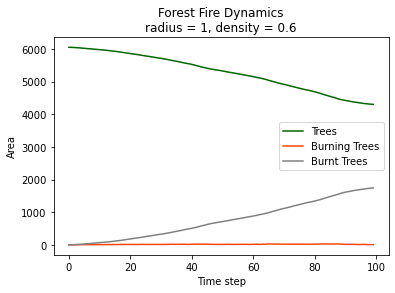
\includegraphics[width=0.5\textwidth,height=\textheight]{../plots/r1d6.png}
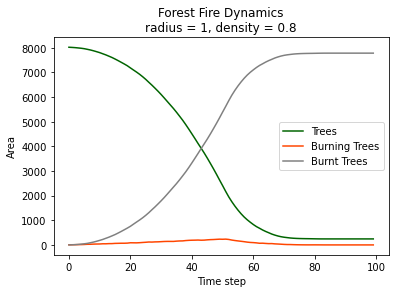
\includegraphics[width=0.5\textwidth,height=\textheight]{../plots/r1d8.png}
\textbf{Figure 1:} Summary plot of Forest Fire CA overtime with an
individual probability of fire of \(q = 0.5\) with a neighborhood of
radius 1 with differing initial forest densities (\(d = 0.6\)
\emph{left}; \(d = 0.7\) \emph{right}). Lines are cummulative areas for
the three states: trees, burning trees, and burnt trees (mean of five
stochastic trials).

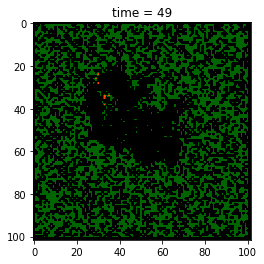
\includegraphics[width=0.5\textwidth,height=\textheight]{../plots/ForestPlot_d6r1.png}
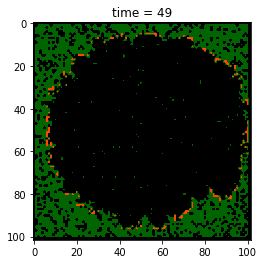
\includegraphics[width=0.5\textwidth,height=\textheight]{../plots/ForestPlot_d8r1.png}
\textbf{Figure 2:} Snapshot of the Forest Fire CA with a radius of one
during a run at t = 49 with initial densities of \(d = 0.6\) \emph{left}
and \(d = 0.8\) \emph{right}.

\hypertarget{radius-three}{%
\subsubsection{Radius Three}\label{radius-three}}

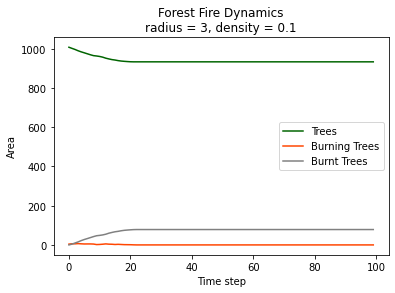
\includegraphics[width=0.5\textwidth,height=\textheight]{../plots/r3d1.png}
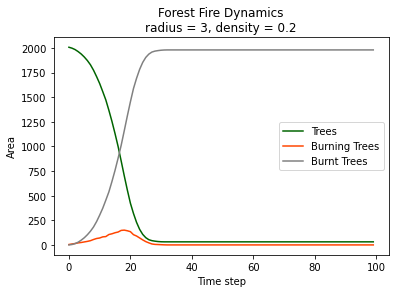
\includegraphics[width=0.5\textwidth,height=\textheight]{../plots/r3d2.png}
\textbf{Figure 3:} Summary plot of Forest Fire CA overtime with an
individual probability of fire of \(q = 0.5\) with a neighborhood of
radius 3 with differing initial forest densities (\(d = 0.1\)
\emph{left}; \(d = 0.2\) \emph{right}). Lines are cummulative areas for
the three states: trees, burning trees, and burnt trees (mean of five
stochastic trials).

\pagebreak

\hypertarget{part-2-diffusion-limited-aggregation-dla}{%
\section{Part 2: Diffusion-Limited Aggregation
(DLA)}\label{part-2-diffusion-limited-aggregation-dla}}

We implemented a diffusion-limited aggregation (DLA) model in python to
simulate the formation of a snowflake from randomly diffusion water
vapor particles as they collide with a frozen ice crystal `seed' and
freeze onto it. See \texttt{Snowflake\_DLA.py} for the model code. In
our model we have an adjustable n by n grid of cells (where n is odd)
with periodic boundaries, where cells can take one of three states:
empty (0), randomly floating particle (1), or frozen seed (2).

We initialize the model with empty cells apart from a frozen seed in the
central cell. We then add water vapor particles to a random subset of
the outermost border of cells, with an adjustable probability d. We use
synchronous updates to update the system according to the following
rules:

\begin{itemize}
\tightlist
\item
  If a floating particle is touching a frozen cell, it will freeze in
  its current position.
\item
  If it doesn't freeze, it will move up, down, left or right with equal
  probability.
\item
  Frozen cells will stay frozen.
\end{itemize}

We then add more random particles to the border again after each update,
and observe the system periodically. We did not speed it up with gravity
or variable step length, so it runs quite slowly.

To get a nice snowglobe effect with swirling particles that can run
quickly, we ran the model for \(75\) timesteps on a \(15 x 15\) grid,
adding particles with probability \(d = 0.1\). However, with such a
small grid, individual cells are relatively large, and it is hard to get
a pretty fractal, especially as the snowflake tends to freeze out to the
edges, locking up the border cells and preventing new particles from
drifting in.

To get a nice snowflake fractal we ran the model for \(24,000\)
timesteps on a \(55 x 55\) grid, adding snowflakes with a probability
\(d = 0.0001\), observing the system every 1000 time steps. The larger
grid and smaller cells helped to make a lacier fractal that could grow
without bumping into edges and freezing the incoming particles.

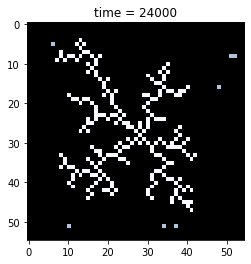
\includegraphics[width=0.5\textwidth,height=\textheight]{../plots/Snowflake.png}
\textbf{Figure 3: One of the world's prettiest digitial snowflakes
generated by our diffusion-limited aggregation.}

\pagebreak

\hypertarget{part-3-gamblers-ruin}{%
\section{Part 3: Gambler's Ruin}\label{part-3-gamblers-ruin}}

\hypertarget{probability-of-winning-the-game}{%
\subsection{Probability of winning the
game}\label{probability-of-winning-the-game}}

\hypertarget{set-up}{%
\subsubsection{Set up}\label{set-up}}

\begin{itemize}
\item
  Suppose you are flipping a biased coin with probability of heads:
  \(p\).
\item
  You begin the game with an intial \(0 < z < W\) dollars. If it is
  heads you gain a dollar, if it is tails you lose a dollar. The game
  will end if you run out of money or hit the target of \(W\) dollars.
\item
  \(S_n\) is the amount of money you have in round \(n\).
\item
  \(T = min\{n : S_n = 0, S_n = W\}\) So T is the number of rounds it
  takes for you to reach \$0 or \$\(W\), which is when the game ends
\end{itemize}

\hypertarget{what-is-the-probability-that-you-will-eventually-win-prove-your-conclusion-with-rigorous-arguments.}{%
\subsubsection{\texorpdfstring{\textbf{What is the probability that you
will eventually win? Prove your conclusion with rigorous
arguments.}}{What is the probability that you will eventually win? Prove your conclusion with rigorous arguments.}}\label{what-is-the-probability-that-you-will-eventually-win-prove-your-conclusion-with-rigorous-arguments.}}

To begin, similar to the random walk in class, we must first consider
the probability of the first step. If \(P_z\) is the probability of
having your initial value of \(z\) then the probability of being one
dollar below or above can be determined by \(p\) and \((1-p)\):

\[P_z = pP_{z+1} + (1-p)P_{z-1}\]

To solve for the chance that you have gained a dollar \(P_{z+1} - P_z\)
you may substitute \(P_z\) as \(pP_z + (1-p)P_z\).

\[
\begin{aligned}
pP_z + (1-p)P_z &= pP_{z+1} + (1-p)P_{z-1} \\
pP_{z+1} - pP_z &= (1-p)P_z - (1-p)P_{z-1} \\
p(P_{z+1} - P_z) &= (1-p)(P_z - P_{z-1}) \\
P_{z+1} - P_z &= \frac{1-p}{p}(P_z - P_{z-1}) \\
\end{aligned}
\]

We can simplify this for \(P_2 - P_1\) using the fact that \(P_0 = 0\).
If we then simplify for \(P_3 - P_2\) and substitute in \((P_2 - P_1)\),
we can see a recursive pattern, which can be generalized as:

\[P_{z+1} - P_z = (\frac{1-p}{p})^z P_1\]

\[
\begin{aligned}
P_{z+1} - P_z &= \sum_{n=1}^{z} (P_{n+1} - P_n) \\
              &= \sum_{n=1}^{z} (\frac{1-p}{p})^n P_1 \\
      P_{z+1} &= P_1 + P_1\sum_{n=1}^{z} (\frac{1-p}{p})^n \\
              &= P_1\sum_{n=0}^{z} (\frac{1-p}{p})^n \\
\end{aligned}
\]

Since this is a geometric series, we can use a geometric series equation
to simplify it to the following:

\[ P_{z+1} = P_1 \frac{1-(\frac{1-p}{p})^{z+1}}{1-\frac{1-p}{p}} \]

We can then consider a value of \(z\) just one below the target \(W\) so
that \(z = W - 1\). And using the definition \(P_W = 1\) (\emph{i.e.}
the probability of winning at \(W\) is 1 by definition) we can get the
equation:

\[ P_W = 1 = P_1 \frac{1-(\frac{1-p}{p})^W}{1-(\frac{1-p}{p})} \]

We used this to solve for \(P_1\), which is as follows:

\[ P_1 = \frac{1- \frac{1-p}{p}}{1 - (\frac{1-p}{p})^W} \]

This expression for \(P_1\) can be substited into the equation for
\(P_{z+1}\) and simplified to get the following:

\[ P_z =  \frac{1-(\frac{1-p}{p})^z}{1-(\frac{1-p}{p})^W} \]

\hypertarget{probability-of-a-never-ending-game}{%
\subsection{Probability of a never-ending
game}\label{probability-of-a-never-ending-game}}

\textbf{Prove that \(Pr(T = \infty) = 0\)}

\[
\begin{aligned}
Pr(T = \infty) &= \frac{\text{\# of infinite paths}}{\text{all paths}} \\
&= \frac{\text{\# of paths that never reach 0 or W}}{\text{all paths}} \\
&= \frac{\text{(all paths)} - \text{(\# winning paths)} - \text{(\# losing paths)}}{\text{all paths}} \\
\end{aligned}
\]

Probability of winning is \(> 0\) if \(i\) is \emph{not equal to} \(0\)
as we saw in the previous question

numerator \(<\) all paths

Denominator = All paths = \(2^T\)

As \(T \rightarrow \infty\): denominator = \(2^T \rightarrow \infty\),
and the whole fraction \(\rightarrow\) \(0\)

So \(Pr(T = \infty) = 0\)

This shows that our friend is either very generous or very devious
depending on how the coin is biased.

\end{document}
